%needs Packages:
% - \usepackage[export]{adjustbox} for  "valign=t"

\section{Wichtige Funktionen}
\begin{tabular}{p{5cm} p{12.5cm}}
  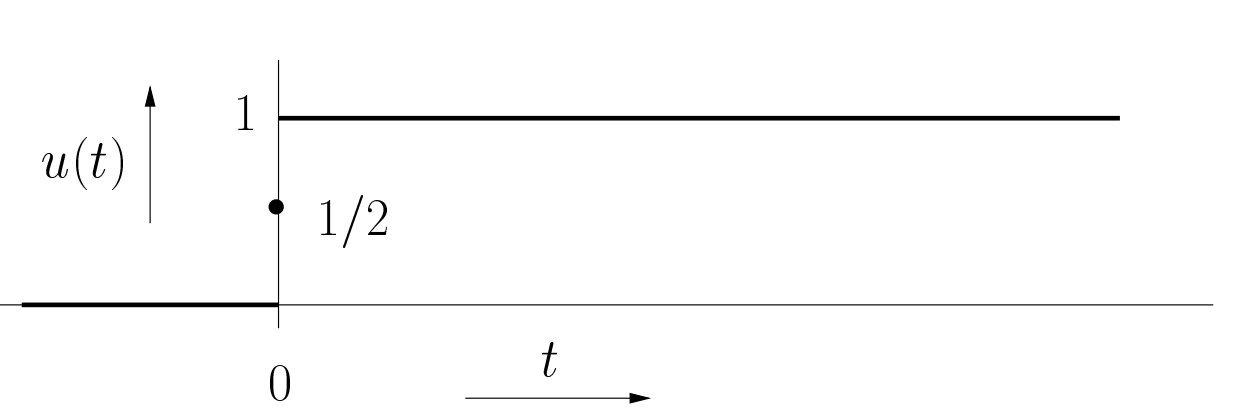
\includegraphics[width = 5cm, valign=t]{include/Wichtige Funktionen/img/Sprungfunktion.png} &
  Sprungfunktion (Heaviside):
  Normierter Einschaltvorgang
  $$H(t) = \begin{cases}
               0 \textrm{ für }  t<0,                                                                      \\
               [\frac{1}{2} \textrm{ für }  t = 0,] \textrm{ \tiny(nicht immer vorhanden; dann 1 für t=0)} \\
               1 \textrm{ für }  t >0.
             \end{cases}   $$
  \\
  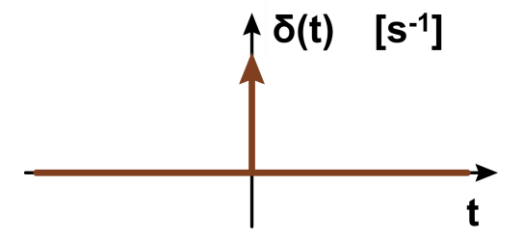
\includegraphics[width = 5cm, valign=t]{include/Wichtige Funktionen/img/Impulsfunktion.png} &
  Diracimpuls \tiny (auch Impuls-/Deltafunktion, Delta-Distribution)
  \normalsize \newline
  Unendlicher kurzer normierter Impuls mit unendlicher Amplitude
  $$\int\limits _{-\infty} ^{+\infty} f(t) \cdot \delta (t-t_0) dt = f(t_0) \;
    \int\limits _{-\infty} ^{+\infty} f(t) \cdot \delta (t) dt = f(0) \;
  \int\limits _{-\infty} ^{+\infty} \delta (t) dt = 1$$                                 \\
  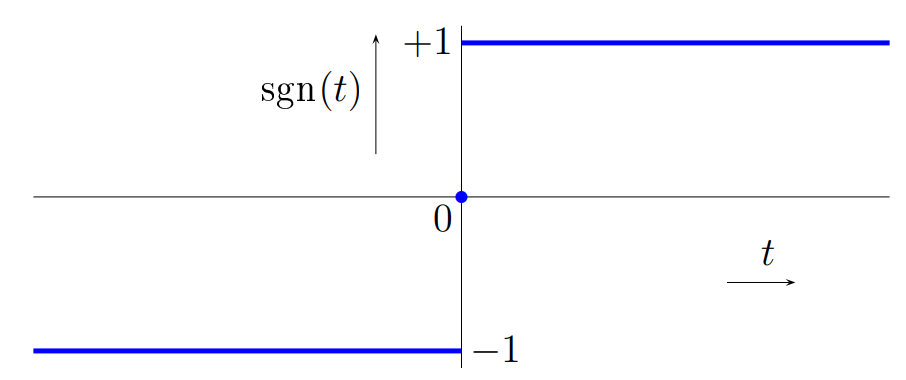
\includegraphics[width = 5cm, valign=t]{include/Wichtige Funktionen/img/Signumfunktion.png} &
  Signumfunktion (Vorzeichenfunktion)
  $$sgn(t) = \begin{cases}
                 -1 \textrm{ für }  t<0,  \\
                 0 \textrm{ für }  t = 0, \\
                 1 \textrm{ für }  t >0.
               \end{cases}   $$                                                   \\
  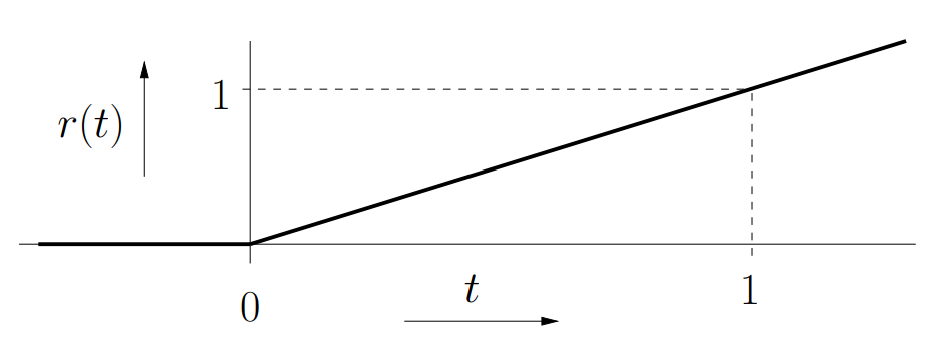
\includegraphics[width=5cm, valign=t]{include/Wichtige Funktionen/img/Rampenfunktion.png}   &
  Rampenfunktion 
  $$r(t) = \begin{cases}
               0 \textrm{ für } t \leq 0, \\
               t \textrm{ für } t > 0.
             \end{cases}$$\\
\end{tabular}
